% !TEX root = ../main.tex

\section{What is Blockchain Technology?}
\label{sec:blockchain}

\begin{figure*}
	\centering
	\includegraphics[page=2,scale=.75]{figures/grounded-theory-main}
	
	\caption{Technical Properties for Blockchain Technology}
	\label{fig:technical-properties}
\end{figure*}

\begin{figure}
	\centering
	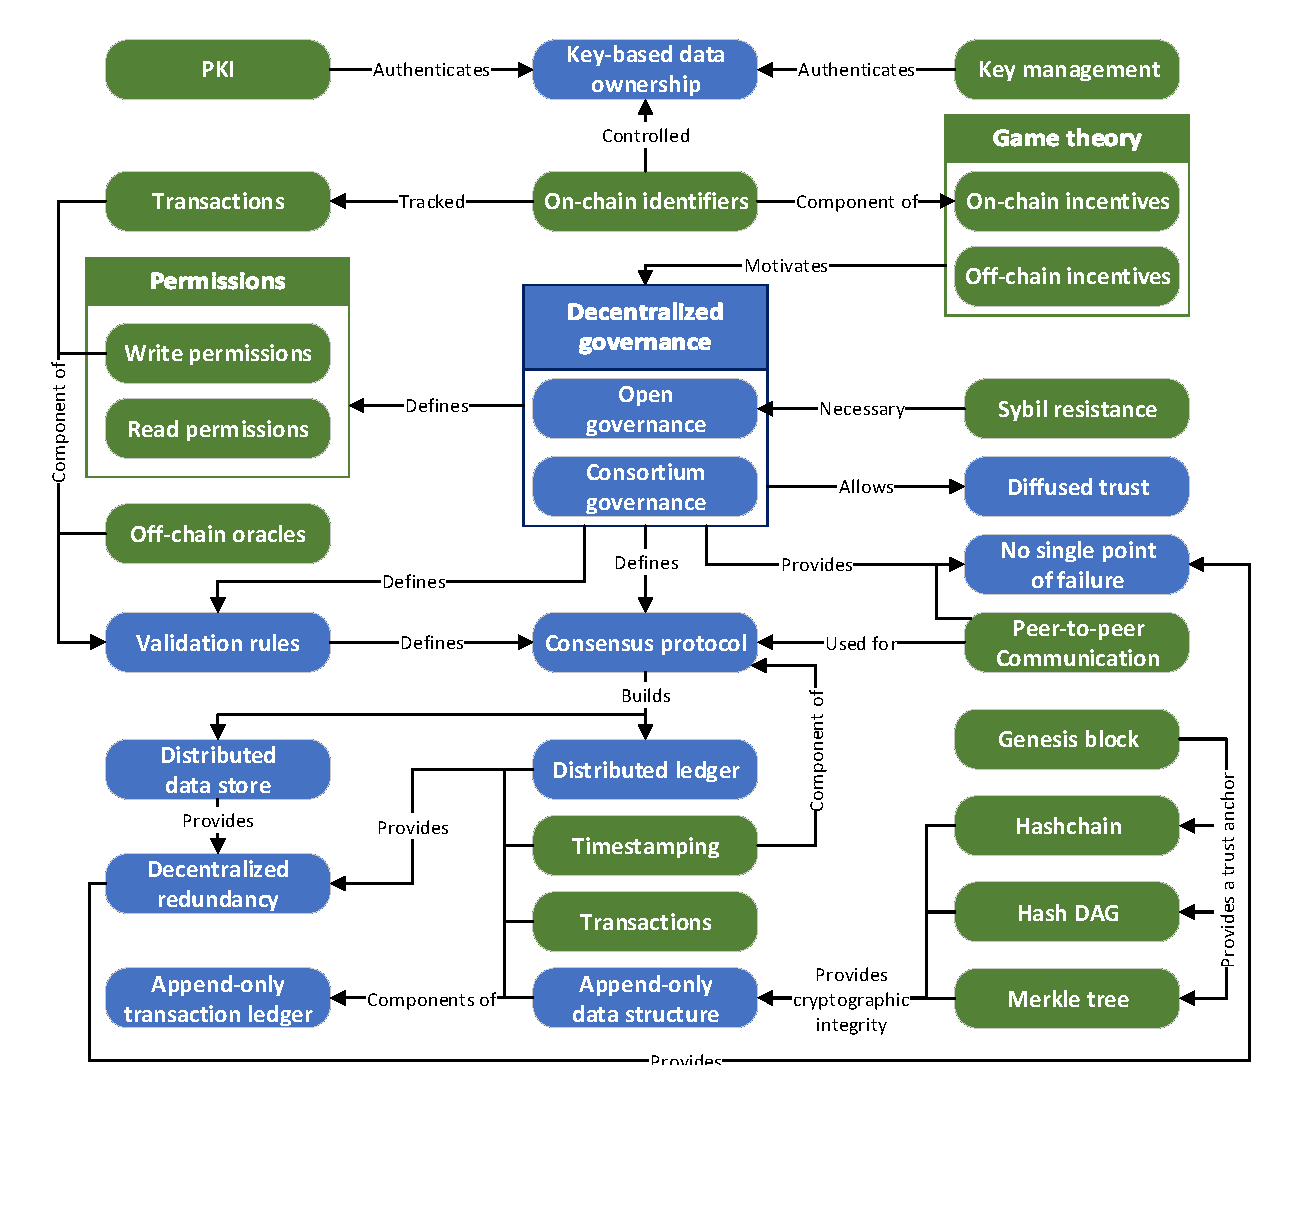
\includegraphics[page=1,scale=.75]{figures/grounded-theory-main}
	
	{\small Blue---technical properties, green---technical primitives}
	\caption{Technical Properties and Primitives for Blockchain Technology}
	\label{fig:technical-properties-full}
\end{figure}

Our literature analysis finds three key groupings of technical properties related to Blockchain technology (see Figure~\ref{fig:technical-properties}; Figure~\ref{fig:technical-properties-full} shows how these properties are related to various technical primitives).
Most importantly, consensus is used to provide \textit{shared governance and operation}.
In support of shared governance and operation, other technical properties provide \textit{verifiable state} and {resilience to data loss}.
By themselves, these property groups are nothing new, but used together they define \emph{Blockchain technology}, or \emph{Blockchain} for short.
In Section~\ref{sec:distributed-comparison} we describe how other distributed technologies compare to Blockchain technology.

\subsection{Shared Governance and Operation}
\label{sec:sharedgov}

%Before describing how shared governance and operation defines Blockchain technology, it is important to define both of these concepts.
%Governance is the process by which one or more entities (e.g., an individual, a company, a government agency) define how a system will operate---i.e., what operations are supported and how those operations function.
%Governance can be singular---a single entity (e.g., a developer, a company) defines the system---or it can be shared---multiple entities work together to define the system (e.g., IETF, RFC).
%Operation refers to the number of parties that actually operate a system.
%Operation can be singular---a single entity executes the system (e.g., a trusted third party)---or shared---multiple entities collectively operate the system (e.g., through the use of a consensus protocol).
%Note, distributed operation (i.e., operation on many machines) does not imply shared operation, as the owner/operator of all distributed nodes may still be a single entity.

Blockchain technology was created to address the scenario in which a collection of parties----referred to hereafter as \emph{miners}---want to participate in a communal system but do not trust each other or any third party to operate the system singlehandedly.
By participating in both the governance and operation of the system (i.e., shared governance and operation), each miner can be assured that the system is operating correctly.
Even if some of the miners become compromised, the uncompromised miners retain the ability to detect malicious actions by the compromised miners and to prevent them from interfering with the correct operation of the system.
In this regard, Blockchain technology provides \emph{diffused trust} wherein it is not individual miners but rather the collective of all miners that is trusted.\footnote{This property has often been called ``trustlessness''; this is incorrect as trust still exists but has simply been diffused among multiple parties.}

Shared operation is enabled by the use of \emph{consensus protocols}, which are used by the miners to agree upon which operations---known as \emph{transactions}---will be executed by the system.
The consensus protocols allow miners to view transactions and validate that the system is operating appropriately, an important consideration as the miners do not trust that only valid transactions will be submitted to the consensus protocol.
Shared governance is provided by the ability of miners to configure their clients to only approve the transactions they believe are acceptable, effectively allowing them to vote for how the system should function.
If there is disagreement regarding system functionality, it is possible for a Blockchain-based system to split, resulting in the creation of competing systems that include only a subset of each other's transactions.
Usually these forks are temporary, with miners either choosing to all adopt the same rules, but it is possible for a fork to result in the permanent creation of two non-interoperable Blockchain systems (e.g., Bitcoin Classic and Bitcoin Cash).

%In Blockchain systems that use a majority-voting consensus mechanism for transaction validation, there are two types of forks that can occur.
%In a soft fork, transactions that validate with the modified rules will also validate with the original rules, but transactions that validate with the original rules might not validate with the modified rules.
%In a hard fork, transactions that validate with the modified rules will not necessarily validate with the original rules.
%The benefit of a soft fork is that both sets of miners can continue participating in the first consensus protocol, with transactions following the modified rules always being accepted and the transactions following the original rules only being accepted if there is a majority of miners who still use the original rules.
%While a soft fork is not a permanent situation, it can provide time for miners to slowly adopt the modified protocol while allowing both sets of miners to operate on the same data.

Blockchain systems can be categorized based on who is allowed to act as a miner:\footnote{In our coding, we also identified the concept of private governance, which eschews the notion of miners. This concept is discussed later in Section~\ref{sec:private-blockchain}.}

\begin{itemize}
	\item \emph{Open governance (i.e., permissionless Blockchains).}
	Any party that is willing to participate in the consensus protocol is allowed to do so.
	These systems are susceptible to Sybil attacks, so it is necessary for them to use consensus protocols in which miners prove ownership and/or expenditure of some finite resource rather than relying on proofs of identity.
	Proof-of-work~\cite{DN93,back1997partial,NakamotoS8} (demonstrating ownership of computing resources) and proof-of-stake~\cite{Bano17,garay2018consensus} (demonstrating ownership of digital assets stored by the Blockchain system) are the most common methods.
	
	\item \emph{Consortium governance (i.e., permissioned Blockchains).}
	Only approved miners that can attest to their identity are allowed to participate in the consensus protocol.
	The starting set of approved miners is defined at system initialization.
	If this set never changes, it is known as a \emph{static consortium}.
	Alternatively, in an \emph{agile consortium} miners change over time, either based on the rules of the system (e.g., random selection) or through consensus by the existing miners.
	Because miners in a consortium have known identities, they can use Byzantine fault tolerance-based consensus protocols, which do not require the resource expenditure of the Sybil-resistant protocols used in open governance-based systems~\cite{Bano17,garay2018consensus}.		
\end{itemize}

For each type of governance, there is a need to incentivize correct participant behavior.
The first type of incentive is an \emph{intrinsic incentive}---i.e., miners maintain the system faithfully because they derive value from using it.
Next, \emph{on-chain incentives} exist when the Blockchain system provides direct benefits to miners for faithful execution (e.g., minting currency and giving it to the miners).
Finally, \emph{off-chain incentives} are any incentive that is not managed by the Blockchain system---for example, contractual obligations or individual reputation.
Importantly, off-chain incentives only apply to consortium governance as they inherently rely on knowing the identity of the miners.

%Note, the literature sometimes refers to open and consortium governance Blockchain systems as \emph{permissionless} and \emph{permissioned} Blockchains, respectively.
%We avoid this terminology as it can be confusing to readers.
%For example, an open governance Blockchain system can still implement permissions for how users can interact with assets tracked by the Blockchain; this is confusing if the system is also referred to as ``permissionless''.

\subsection{Verifiable State}
Miners adopt Blockchain technology because they want their trust to be rooted in the system---i.e., that the current state of the system accurately reflects the transactions that the consensus protocol allowed to execute in the past.
To enable this trust, Blockchain technology writes all transactions to a cryptographically-verified append-only ledger ~\cite{tamassia2003authenticated}, providing full system provenance and allowing miners (or outside parties) to audit the system's current state and past operations.
In many systems, including Bitcoin, this ledger is colloquially referred to as the ``blockchain'', but we avoid that term as it unnecessarily confusing to discuss both Blockchain (big-B) technology and the blockchain (little-b) data structure.

The first entry in the append-only ledger is known as the \emph{genesis block}.
The genesis block is responsible for specifying the initial parameters for the system.
Whenever a new transaction is approved by the miners, it is added to the ledger and cryptographically linked to one or more preceding transactions (or the genesis block for the first transaction)~\cite{bayer1993improving,haber1990time,haber1997secure}---for example, by signing the concatenation of the latest transaction and a hash of the transactions it is linked to.
The resulting data structure can be either linear (e.g., Bitcoin's hash chain) or branching (e.g., a Merkle tree or directed acyclic graph).
Regardless of the underlying structure, it is critical that all transactions are strictly ordered and that this ordering never changes after consensus is reached.

%Transactions stored in the append-only ledger can contain any data allowed by the consensus protocol, but in practice transactions are usually concerned with \emph{tokens}.
%Tokens represent a resource that is either on-chain (e.g., cryptocurrency, a document) or off-chain (e.g., a diamond, a file stored in the cloud) and are used to track that resource within the Blockchain system.
%For off-chain assets, there needs to be the ability to \emph{staple} the on-chain token to the off-chain assets.
%While there have been a variety of proposals for doing this (e.g., etching the token's identifier onto the physical items), effective stapling remains a challenge (see Section~\ref{sec:challenges}).

\subsection{Resilience to Data Loss}
If the ledger was only stored in a single location, deleting or modifying that data store could be detected by all parties, but there would be no guarantee that the data could be restored.
In Blockchain technology, the ledger is replicated among miners to address this single point of failure.
When data does need to be restored---for example, when an individual miner's ledger was corrupted---the replicated data can be verified to ensure that it correctly represents the system state.

%The cryptographically-authenticated append-only ledger is replicated among a set of miners and this replication is important for several reasons.
%First, during the consensus protocol it is necessary for miners to be aware of previous transactions that might invalidate the transaction being considered for approval.
%Second, it removes a single point of failure, preventing the loss of data at one site from impacting the overall system.
%Third, it protects against malicious attempts to modify the append-only ledger.
%Without replication it would still be possible to detect that data had been corrupted, but there is no guarantee that the original data could be restored.

%The use of a cryptographically authenticated ledger also has the benefit that it is possible to verify that the current state properly proceeds from the initial genesis block.
%While this is useful for runtime integrity checks, it is also useful when a miner needs to rebuild their state.
%In this case, they can replicate data from another miner and verify its authenticity without the need to trust the other miner as would be required in most distributed databases.

Some Blockchain systems try to limit the amount of data any given miner needs to replicate by segmenting the data and assigning miners to handle governance and operations for only a subset of the system.
This is known as \emph{sharding}, with individual segments of the data known as \emph{shards}.
Sharding can drastically reduce the amount of data that miners need to store while also increasing the performance of the consensus protocol, which often scale based on the number of miners.
Still, sharding comes with the drawback that miners are no longer able to audit the system as a whole.
Additionally, by reducing the number of miners responsible for any given transaction, sharding also reduces the number of miners an adversary would need to compromise to attack that transaction.

\section{What are Blockchain Technology's Capabilities?}
\label{sec:capabilities}

\begin{figure*}
	\centering
	\includegraphics[page=4,scale=.75]{figures/grounded-theory-main}
	
	{\small Purple---capabilities, blue---technical properties, green---technical primitives. Arrows indicate that the destination depends on the source.}
	\caption{Capabilities for Blockchain Technology}
	\label{fig:Capabilities}
\end{figure*}

Capabilities define the high-level functionality that can be achieved by using Blockchain technology in a system's design.
Blockchain's three core capabilities were described in the preceding section: (1) shared governance and operation, (2) verifiable state, and (3) resilience to data loss.
In our coding, we identified 11 additional capabilities (see Figure~\ref{fig:Capabilities}).

\paragraph{Provenance and Auditability}
Blockchain systems provide a complete history of all transactions that were approved by the consensus process (i.e., full-system provenance).
%While failed transactions are not normally written to the ledger, they could be if needed by the system for auditability.
This information can be used by the miners to audit the system and ensure that it has always followed the appropriate rules.
Additionally, this information can be used by non-miners to verify that the system is being governed and operated correctly.

If transactions are used to store information regarding digital or real-world resources, the resources must be \emph{stapled} to on-chain identifiers. Then the provenance information for the Blockchain system can also be used to provide audit information for those resources.
This can be used to track physical, off-chain assets (e.g., for supply chain management), digital, off-chain assets (e.g., copyrighted digital media), or digital, on-chain assets (e.g., cryptocurrencies or data files).
 
\paragraph{Access Control and Pseudonymity}
Data stored in a blockchain may have limitations regarding which users can use it as an input to a transaction or modify it as part of the operation of the transaction.
For example, a financial asset should only be a valid input to a transaction if the owner of that asset approves its use.
One approach to providing this functionality is storing access control lists (ACLs) in the blockchain and having the appropriate users prove their identity to the miners (e.g., using Kerberos or OAuth 2.0) as part of the transaction validation process.

More commonly, access control in a blockchain system is implemented cryptographically: data is associated with a public key when it is created and the ability to use or modify this data as part of transaction is granted only to users that can prove knowledge of the corresponding private key (e.g., by generating a signature over the transaction that validates with the public key attached to the data).
Ownership of the data can be expanded or transferred by associating it with a new public key.

On key benefit of access control using Blockchain is that the provenance of access control is automatically recorded.
This means that a full record of not only a user's permissions, but how they received those permissions, is stored.
This information can be used to automatically revoke permissions if it is discovered that a user was granted these permissions by a compromised account---for example, when a malicious insider grants inappropriate permissions to other insiders.

Key-based (as opposed to ACL-based) ownership of data has another advantage: it allows for pseudonymous ownership and use of data.
Still, this requires careful attention in the system design to use appropriate cryptographic techniques (e.g., zero-knowledge proofs, mix networks, or secure multi-party computation) to avoid linking real-world individuals to their keys and actions. This remains an open problem.

\paragraph{Automatic Execution (Smart Contracts)}
Blockchain transactions can also represent and store executable functions known as \emph{smart contracts}.
These smart contracts can be executed automatically in response to a function call in later transactions, with both the inputs and outputs of the function recorded within the calling transaction.
The smart contracts themselves are executed by the miners with outputs being verified through the consensus protocol.
The computational power of these scripts is determined by the system's rules, ranging from supporting only basic functionality (e.g., verifying a signature in Bitcoin) to providing Turing-complete functionality (e.g., Ethereum).

Smart contracts benefit from Blockchain technology's other capabilities (e.g., shared operation, auditability, and resilience).
For example, multiple miners execute and verify the output of a smart contract to help ensure that an adversary is unable to tamper with the result of a function.
Similarly, the ability to audit inputs and outputs can be used to attribute incorrect usage of a smart contract.
Still, smart contracts suffer from problems common to all programs (e.g., bugs, security flaws, complexity, or non-termination) and a failure to recognize this reality can lead to disastrous consequences.\footnote{This is best exemplified by the debate over ``code is law'' and the DAO attack: \url{https://www.coindesk.com/understanding-dao-hack-journalists/}.}

\paragraph{Data Discoverability}
If users are allowed to read any record in a Blockchain's distributed data store, then it is trivial to search for records of interest.
This capability is nothing more than what is provided by having a read-only data lake, but still it was frequently discussed in the literature we reviewed.